\newchapter{Einleitung}
\label{kap:1}


Partielle Differentialgleichungen sind in vielen Bereichen der Natur- und Ingenieurswissenschaften wiederzufinden. Da die exakte Lösung nicht immer existiert bzw. die Bestimmung solch einer Lösung beliebig komplex werden kann, haben numerische Löser für partielle Differnetialgleichungen in den letzen Jahrzehnten mit der Weiterentwicklung des Computers immer mehr an Bedeutung gewonnen. Die Lösung kann daher mittel \idx{Galerkin-Verfahren} (bzw. Finiter-Elemente-Methode\index{Finite-Elemente-Methode}) vollzogen werden. Hierbei wird die eigentliche Differentialgleichung nur noch approximativ auf einem Gitter gelöst, wobei wir durch Verfeinerung des Gitters die Genauigkeit der Lösung erhöhen, was allerdings auch zu höherem Rechenaufwand führt. Daher ist es sinnvoll die Verfeinerung des Gitters zu steuern, so dass möglichst wenig, aber für eine hinrechend genaue Lösung noch genügend Elemente verfeinert werden. Diese Verfahren werden als \textit{\idx{adaptive Verfeinerungsstategie}n} bezeichnet und sind im Allgemeinen von der Form:
\[
	\text{solve}\ \ \ra \ \ \text{estimate}\ \ \ra\ \ \text{mark}\ \ \ra\  \ \text{refine} \, .
\]
Da die exakte Lösung in den meisten Fällen nicht bekannt ist, ist der Schritt "`estimate"' von entscheidender Bedeutung. Hierbei wird der Fehler zur exakten Lösung auf dem nächsten Gitter mittels eines a posteriori Fehlerschätzer bzgl. des aktuellen Gitters abgeschätzt, was Zuverlässigkeit und Effektivität des Schätzers voraussetzt, d.h. durch Verkleinerung des Fehlerschätzers sollte sich auch der exakte Fehler verringern. Im Schritt "`mark"' wählen wir dann genau die Elemente aus, die bzgl. des gewählten Schätzers einen hohen lokalen Anteil an diesem haben.

Dies soll der Mittelpunkt dieser Arbeit sein und wird in Kapitel \ref{kap:4} ausführ-lich behandelt. Allerdings wollen wir dieses Verfahren für einen hierarchischen Fehlerschätzer auf eine partielle Differentialgleichung unter einer Nebenbedingung anwenden. Als Modellproblem hierfür dient ein \idx{Hindernisproblem}, was wir in Kapitel \ref{kap:3} näher beleuchten werden. In Abbildung \ref{abb:1.1} ist im Vergleich die Auslenkung einer eingespannten, belasteten Membran, dessen Auslenkung durch die Laplace-Gleichung modelliert werden kann, ohne und mit Nebenbedingung/Hindernis dargestellt.

\begin{figure}[h]
\begin{center}
\subfigure[ohne Hindernis]{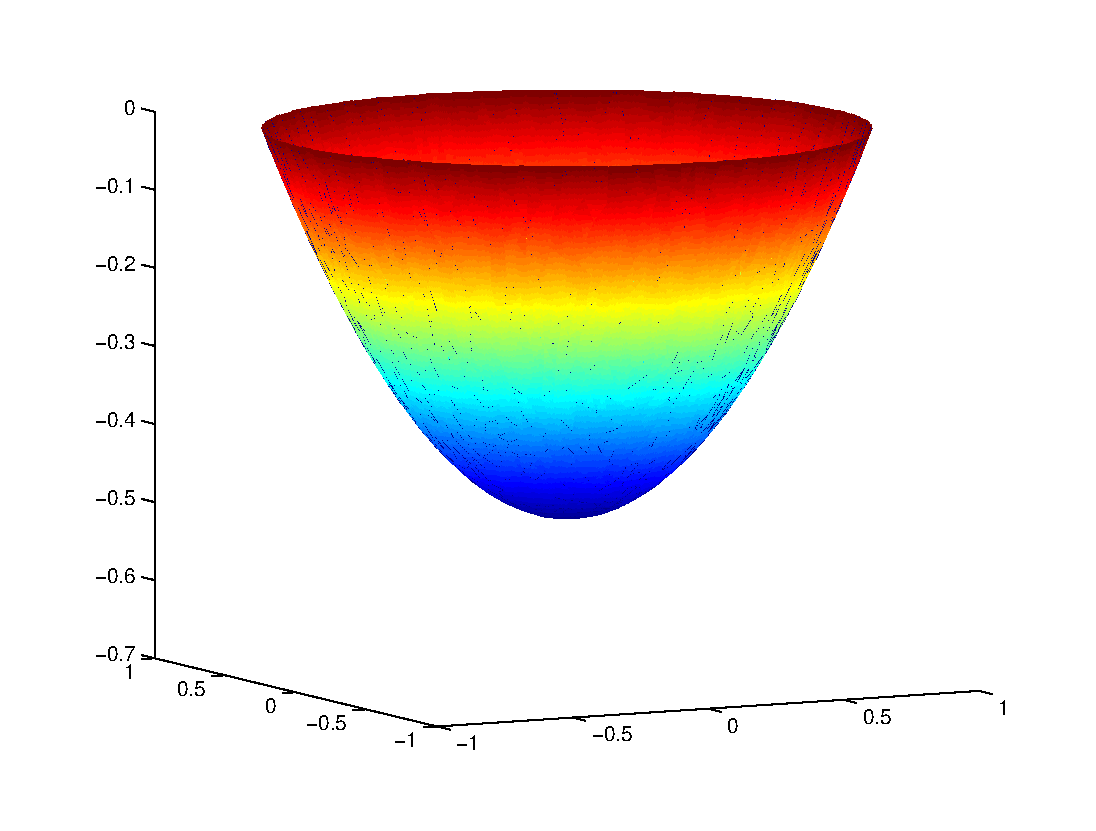
\includegraphics[width=6.25cm]{Abbildungen/bsp_ohne_hindernis.eps}}
\hfill
\subfigure[mit Hindernis: Ebene $z=-0,28$]{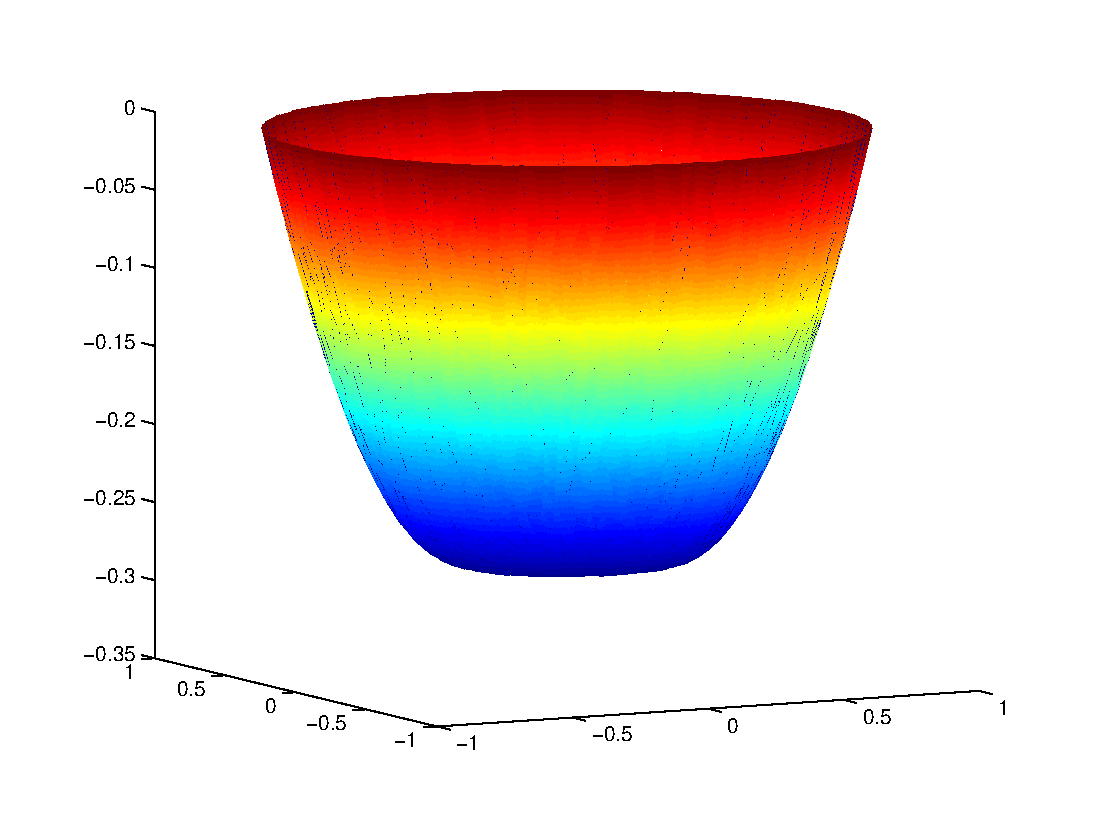
\includegraphics[width=6.25cm]{Abbildungen/bsp_mit_hindernis.eps}}
\end{center}
\caption{Auslenkung einer eingespannten Membran unter Einwirkung einer vertikalen Lastfunktion $f$\label{abb:1.1}}
\end{figure}

Kontaktprobleme sind Probleme aus der Strukturmechanik und stellen eine Anwendung von partiellen Differentialgleichungen unter Nebenbedingung (nämlich der Kontaktbedingung) dar. Diese wollen wir in dieser Arbeit mittels \index{Finite-Elemente-Methode}Finiter-Elemente-Methode untersuchen (Kapitel \ref{kap:3}) und den hergeleiteten Fehlerschätzer aus Kapitel \ref{kap:4} hierauf übertragen.

Die Lösungsverfahren für die adaptive Verfeinerung der Hindernis- bzw. Kontaktproblemen werden wir in Matlab implementieren und die wichtigsten Schritte hierfür in Kapitel \ref{kap:5} darstellen. Letztlich lassen sich diese Implementatierungen zur Validierung der hergeleiteten Resultate aus Kapitel \ref{kap:4} nutzen und wir stellen in Kapitel \ref{kap:6} einige numerische Beispiele vor.
%
%
%\begin{itemize}
%\item Thema (worum geht es?) $\ra$ Fehlerabschätzung $\ra$ analytische Lösung oftmals nicht bekannt und damit Fehlerschätzer interessant
%\item[$\ra$] in FEM soll Lösung genauer mit weniger Rechenzeit sein, daraus folgt Anwendung adaptiver Verfahren mit verschiedenen Fehlerschätzern
%\item Lücke zum neuen (Kontaktproblematik) füllen in dieser Arbeit
%\item[$\ra$] Übertragung unseres Fehlerschätzers auf Kontaktprobleme, wie und warum?! $\ra$ möglicher Grund: Hindernisprobleme beinhalten Kontaktbereiche (später für Kapitel 4 interessant)
%\item[wichtig:] Vorgehen einer adaptiven Verfeinerungsstrategie mit "`solve $\ra$ estimate $\ra$ ...."' umschreiben
%\item Struktur der Arbeit
%\item
%\item partielle Differentialgleichungen kommen in vielen Bereichen der Natur- und Ingenieurwissenschaften vor $\Ra$ da die Lösung nicht immer exakt möglich bzw. auch sehr komplex sein kann, approximierte Löser interessant $\Ra$ FEM $\Ra$ Verfeinerung des Gitters (Erhöhung des Freiheitsgrades) bringt genauere Lösung, aber auch mehr Rechenaufwand $\Ra$ so wenig wie möglich verfeinern, d.h. nach Möglichkeit in den Bereichen, in denen der Fehler zur exakten Lösung besondern groß ist $\Ra$ adaptive Verfeinerungsstrategie, allgemein von der Form:
%\[
%	\text{solve}\ \ \ra \ \ \text{estimate}\ \ \ra\ \ \text{mark}\ \ \ra\  \ \text{refine}
%\]
%\item da die exakte Lösung in den meisten Fällen nicht bekannt ist, ist der Schritt 2 entscheidend. die Abschätzung erfolgt mittels eines a posteriori Fehlerschätzers, der den Fehler im nächsten Schritt mit dem aktuellen vergleicht
%\item dies soll Mittelpunkt dieser Arbeit sein.
%\item häufig werden PDE allerdings mit Nebenbedingungen betrachtet, was mittels FEM nicht mehr auf ein LGS führt. 
%\item ein modellproblem hierfür ist das hindernisproblem.
%\item anhand dieses wollen wir einen a posteriori Fehlerschätzer herleiten und dessen Effektivität und Zuverlässigkeit auch an numerischen Beispielen validieren
%\item Kontaktprobleme stellen eine  Anwendung einer PDE unter Nebenbedingung dar. $\Ra$ wir wollen daher in dieser Arbeit auch diese mittels Lösung der FEM untersuchen und den hergeleiteten Fehlerschätzer hierauf übertragen.
%\item Implementiert werden die Lösungsverfahren jeweils in Matlab.
%\item in Kapitel 2 werden wir zunächst grundlegendes einführen; Kapitel 3 enthält die Theorie zur exakten und numerischen Lösbarkeit der Probleme mit a priori Fehlerschätzungen; Kapitel 4 ist das zentrale Kapitel er Arbeit und leitet den betrachteten Fehlerschätzer her mit Übertragung auf Kontakt; Kapitel 5 soll die wichtigsten Ideen der Implementierung in Matlab erläutern; Kapitel 6 ist die numerische Validierung
%\end{itemize}
%
%
%



\newpage

%%% Local Variables: 
%%% mode: latex
%%% TeX-master: "Skript"
%%% End: 
